%%% Version 3.4 Generated 2022/06/14 %%%
%%% You will need to have the following packages installed: datetime, fmtcount, etoolbox, fcprefix, which are normally inlcuded in WinEdt. %%%
%%% In http://www.ctan.org/ you can find the packages and how to install them, if necessary. %%%
%%%  NB logo1.jpg is required in the path in order to correctly compile front page header %%%

%\documentclass[utf8]{FrontiersinHarvard}

\documentclass[utf8]{FrontiersinVancouver} % for articles in journals

%\documentclass[utf8]{frontiersinFPHY_FAMS} % Vancouver Reference
%Style (Numbered) for articles in the journals "Frontiers in Physics"
%and "Frontiers in Applied Mathematics and Statistics"

%\setcitestyle{square} % for articles in the journals "Frontiers in Physics" and "Frontiers in Applied Mathematics and Statistics" 

\usepackage{url,hyperref,lineno,microtype,subcaption}
\usepackage[onehalfspacing]{setspace}
\usepackage{comment}
\usepackage{todonotes}

\newcommand{\TODO}[1]{\todo[inline]{#1}}

\linenumbers


\def\keyFont{\fontsize{8}{11}\helveticabold }

\def\firstAuthorLast{von Laszewski {et~al.}} 
\def\Authors{Gregor von Laszewski\,$^{1,*}$,
 J.P. Fleischer\,$^{1}$
Robert Knuuti\,$^{1}$
 and Geoffrey. C. Fox\,$^{1}$}

% Affiliations should be keyed to the author's name with superscript
% numbers and be listed as follows: Laboratory, Institute, Department,
% Organization, City, State abbreviation (USA, Canada, Australia), and
% Country (without detailed address information such as city zip codes
% or street names).

% If one of the authors has a change of address, list the new address
% below the correspondence details using a superscript symbol and use
% the same symbol to indicate the author in the author list.

\def\Address{$^{1}$
Biocomplexity Institute,
University of Virginia,
% Town Center Four,
% 994 Research Park Boulevard,
 Charlottesville, VA, 22911, USA
}
% The Corresponding Author should be marked with an asterisk
% Provide the exact contact address (this time including street name and city zip code) and email of the corresponding author

\def\corrAuthor{Gregor von Laszewski, Biocomplexity Institute,
University of Virginia,
Town Center Four,
994 Research Park Boulevard,
 Charlottesville, VA, 22911, USA
}

\def\corrEmail{laszewski@gmail.com}




\begin{document}
\onecolumn
\firstpage{1}

\title {Article Title} 

\author[\firstAuthorLast ]{\Authors} %This field will be automatically populated
\address{} %This field will be automatically populated
\correspondance{} %This field will be automatically populated

\extraAuth{}% If there are more than 1 corresponding author, comment this line and uncomment the next one.
%\extraAuth{corresponding Author2 \\ Laboratory X2, Institute X2, Department X2, Organization X2, Street X2, City X2 , State XX2 (only USA, Canada and Australia), Zip Code2, X2 Country X2, email2@uni2.edu}


\maketitle


\begin{abstract}

%%% Leave the Abstract empty if your article does not require one, please see the Summary Table for full details.
\section{}
For full guidelines regarding your manuscript please refer to \href{https://www.frontiersin.org/guidelines/author-guidelines}{Author Guidelines}.

As a primary goal, the abstract should render the general significance and conceptual advance of the work clearly accessible to a broad readership. References should not be cited in the abstract. Leave the Abstract empty if your article does not require one, please see the Article Types on every Frontiers journal page for full details


\tiny
\keyFont{ \section{Keywords:} deep learning, benchmarking, hyper parameter search, hybrid heterogeneous hyper parameter serach, earthquake forecasting }
% All article types: you may provide up to 8 keywords; at least 5 are mandatory.
\end{abstract}

\section{Introduction}

todo \citep{las-22-arxiv-workflow-cc}

% For Original Research Articles \citep{conference}, Clinical Trial
% Articles \citep{article}, and Technology Reports \citep{patent}, the
% introduction should be succinct, with no subheadings \citep{book}. For
% Case Reports the Introduction should include symptoms at presentation
% \citep{chapter}, physical exams and lab results \citep{dataset}.



\section{Article types}

For requirements for a specific article type please refer to the
Article Types on any Frontiers journal page. Please also refer to
\href{https://www.frontiersin.org/about/author-guidelines#sections}{Author
  Guidelines} for further information on how to organize your
manuscript in the required sections or their equivalents for your
field

% For Original Research articles, please note that the Material and
% Methods section can be placed in any of the following ways: before
% Results, before Discussion or after Discussion.

\section{Manuscript Formatting}

\subsection{Heading Levels}

%There are 5 heading levels

\subsection{Level 2}
\subsubsection{Level 3}
\paragraph{Level 4}
\subparagraph{Level 5}

\subsection{Equations}
Equations should be inserted in editable format from the equation editor.

\begin{equation}
\sum x+ y =Z\label{eq:01}
\end{equation}

\subsection{Figures}

Frontiers requires figures to be submitted individually, in the same
order as they are referred to in the manuscript. Figures will then be
automatically embedded at the bottom of the submitted
manuscript. Kindly ensure that each table and figure is mentioned in
the text and in numerical order. Figures must be of sufficient
resolution for publication. Figures which are not according to the
guidelines will cause substantial delay during the production
process. Please see
\href{https://www.frontiersin.org/guidelines/author-guidelines#figure-and-table-guidelines}{here}
for full figure guidelines. Cite figures with subfigures as figure
\ref{fig:Subfigure 1} and \ref{fig:Subfigure 2}.


\subsubsection{Permission to Reuse and Copyright}

Figures, tables, and images will be published under a Creative Commons
CC-BY licence and permission must be obtained for use of copyrighted
material from other sources (including
re-published/adapted/modified/partial figures and images from the
internet). It is the responsibility of the authors to acquire the
licenses, to follow any citation instructions requested by third-party
rights holders, and cover any supplementary charges.

%% Figures, tables, and images will be published under a Creative
%% Commons CC-BY licence and permission must be obtained for use of
%% copyrighted material from other sources (including
%% re-published/adapted/modified/partial figures and images from the
%% internet). It is the responsibility of the authors to acquire the
%% licenses, to follow any citation instructions requested by
%% third-party rights holders, and cover any supplementary charges.

\subsection{Tables}

Tables should be inserted at the end of the manuscript. Please build
your table directly in LaTeX.Tables provided as jpeg/tiff files will
not be accepted. Please note that very large tables (covering several
pages) cannot be included in the final PDF for reasons of space. These
tables will be published as
\href{https://www.frontiersin.org/guidelines/author-guidelines#supplementary-material}{Supplementary
  Material} on the online article page at the time of acceptance. The
author will be notified during the typesetting of the final article if
this is the case.

\section{Nomenclature}

\subsection{Resource Identification Initiative}

{\bf Organization:} $RRID:SCR_011743$

\section*{Conflict of Interest Statement}

The authors declare that the research was conducted in the absence of
any commercial or financial relationships that could be construed as a
potential conflict of interest.

\section*{Author Contributions}

GvL is the leadauthor and main contributr to this paper. He has
modified and augmented the earthquake paper to include the ability to
execute hyperparameters. 

JPF is a student hthat has contributed to various aspects of the
workflow component of the paper and to a number of executions and
evaluations of experiment runs.

RK has helped togetehr with GVL in teh implementation of the secign of
cloudmesh-sbatch and the porting of the effort to the UVA machine.

GCF is the author of the earthquake code and facilitaties the
interactions with the MLCommons Science Working group as a group
leader of that effort.

\section*{Funding}

Details of all funding sources should be provided, including grant
numbers if applicable. Please ensure to add all necessary funding
information, as after publication this is no longer possible.

\section*{Acknowledgments}

Work was in part funded by the NSF CyberTraining: CIC:
CyberTraining for Students and Technologies from Generation Z with the
award numbers 1829704 and 2200409 and NIST 60NANB21D151T. 
The work was also funded by the \TODO{Department of Energy under the
  grant ???.}
colleagues, institutions, or agencies that aided the efforts of the
authors.

\section*{Supplemental Data}

\href{https://www.frontiersin.org/guidelines/author-guidelines#supplementary-material}{Supplementary
  Material} should be uploaded separately on submission, if there are
Supplementary Figures, please include the caption in the same file as
the figure. LaTeX Supplementary Material templates can be found in the
Frontiers LaTeX folder.

\section*{Data Availability Statement}

The code is all in public domain and available at github at the following locations

\begin{itemize}

\item cloudmesh-cc -- Is a code to control workflows to be executed on
  remote computing
  resources. \url{https://github.com/cloudmesh/cloudmesh-cc}

\item cloudmesh-sbatch -- Is a code to generate batch scripts for
  hyperparameter studies high performance computers so they can be
  executed on different suppercomputers by multiple
  accounts. \url{https://github.com/cloudmesh/cloudmesh-sbatch}

\item cloudmesh -- Cloudmesh is a large collection of repositories for
  accessing cloud and HPC
  resources. \url{https://github.com/orgs/cloudmesh/repositories}

\item mlcommons eartchquake production -- The MLCommons Sceience
  Working group is described at
  \url{https://mlcommons.org/en/groups/research-science/}. This page
  contains the links to the production level earthquake code.

\item mlcommons eartchquake development -- The development version of
  the code is available in this reporitory. It also contains many of
  the analysis scrripts that are not pare of the production code
  hosted by MLCommons \url{https://github.com/laszewsk/mlcommons}.
  
\end{itemize}


% \bibliographystyle{Frontiers-Harvard}

\bibliographystyle{Frontiers-Vancouver} % Many Frontiers journals
% use the numbered referencing system, to find the style and resources
% for the journal you are submitting to:
% https://zendesk.frontiersin.org/hc/en-us/articles/360017860337-Frontiers-Reference-Styles-by-Journal

\bibliography{vonLaszewski-references}


\section*{Figure captions}

%%% max 15 figures abd table, subfig is one figure

%%%  NB logo1.eps is required in the path in order to correctly compile front page header %%%

\begin{figure}[h!]
\begin{center}

\includegraphics[width=10cm]{logo1}% This is a *.eps file
\end{center}
\caption{ Enter the caption for your figure here.  Repeat as  necessary for each of your figures}\label{fig:1}
\end{figure}

\setcounter{figure}{2}
\setcounter{subfigure}{0}
\begin{subfigure}
\setcounter{figure}{2}
\setcounter{subfigure}{0}
    \centering
    \begin{minipage}[b]{0.5\textwidth}
        
\includegraphics[width=\linewidth]{logo1.eps}
        \caption{This is Subfigure 1.}
        \label{fig:Subfigure 1}
    \end{minipage}  
   
\setcounter{figure}{2}
\setcounter{subfigure}{1}
    \begin{minipage}[b]{0.5\textwidth}
        
\includegraphics[width=\linewidth]{logo2.eps}
        \caption{This is Subfigure 2.}
        \label{fig:Subfigure 2}
    \end{minipage}

\setcounter{figure}{2}
\setcounter{subfigure}{-1}
    \caption{Enter the caption for your subfigure here. \textbf{(A)} This is the caption for Subfigure 1. \textbf{(B)} This is the caption for Subfigure 2.}
    \label{fig: subfigures}
\end{subfigure}

\begin{comment}


\begin{figure}[p]
     \centering
     \begin{subfigure}[b]{0.49\textwidth}
        \centering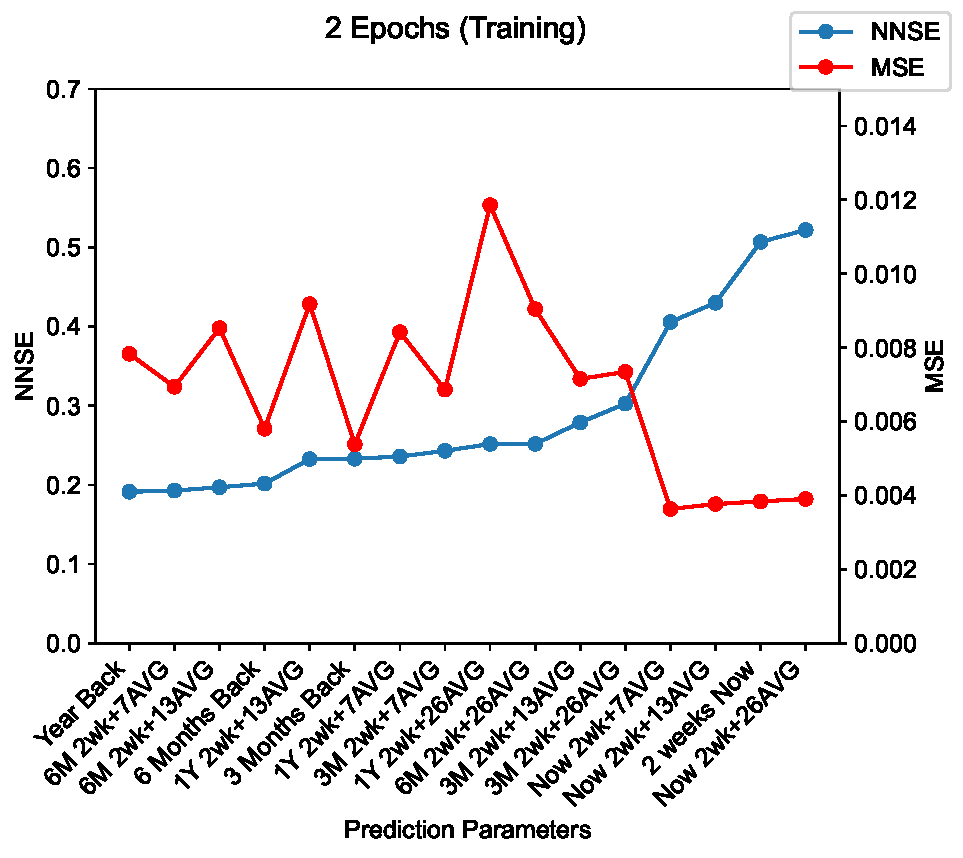
\includegraphics[width=1.0\linewidth]{images/2_training-MSE-and-NNSE.pdf}
        \caption{MSE and NNSE - 2 epochs training}
        \label{fig:tbd1}
     \end{subfigure}
     \hfill
     \begin{subfigure}[b]{0.49\textwidth}
        \centering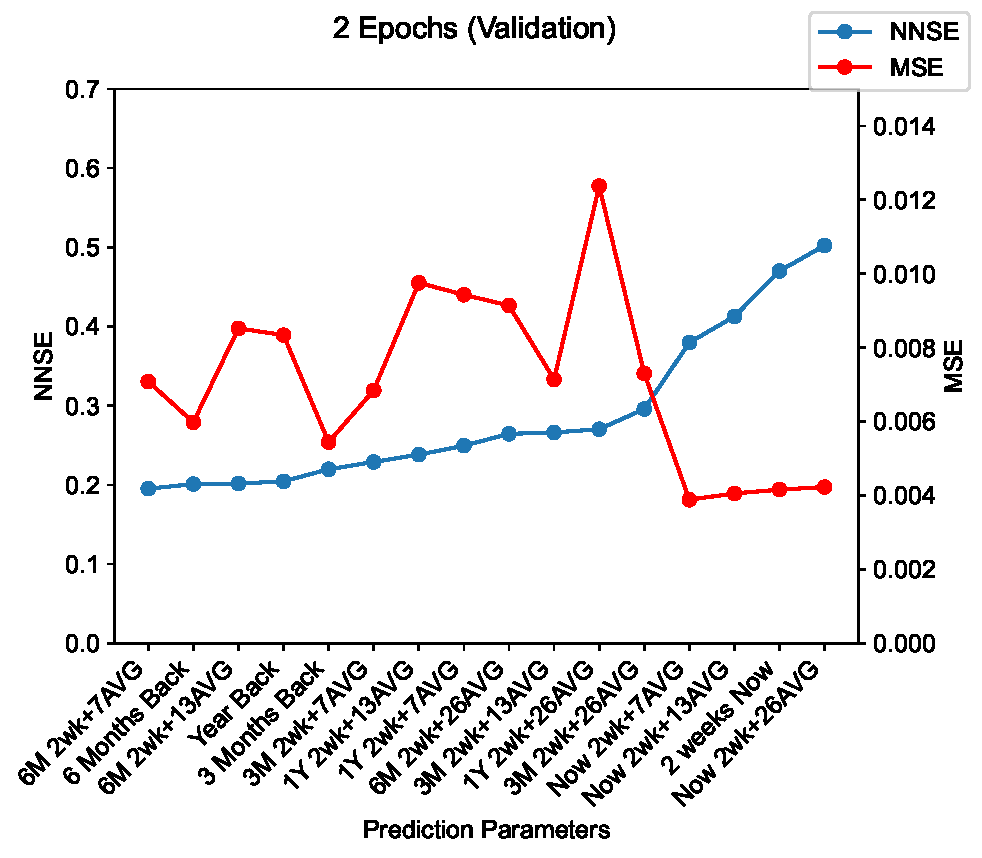
\includegraphics[width=1.0\linewidth]{images/2_validation-MSE-and-NNSE.pdf}
        \caption{MSE and NNSE - 2 epochs validation}
        \label{fig:tbd2}
     \end{subfigure}
     \hfill
     \newline
     \begin{subfigure}[b]{0.49\textwidth}
        \centering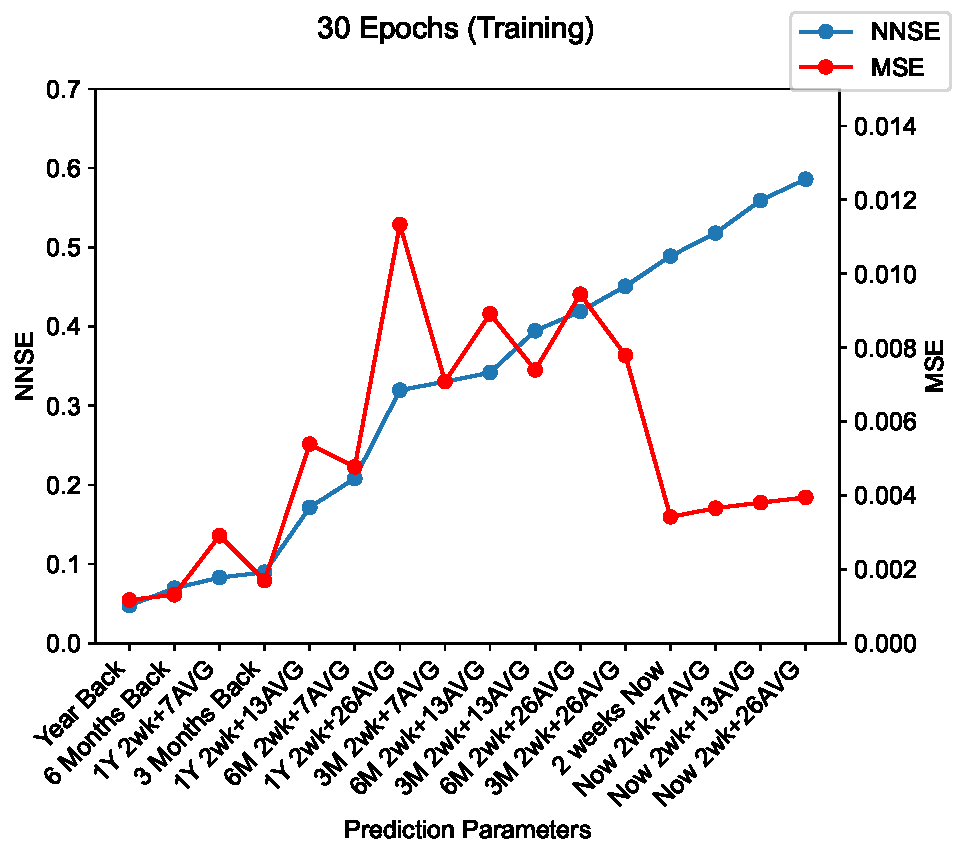
\includegraphics[width=1.0\linewidth]{images/30_training-MSE-and-NNSE.pdf}
        \caption{MSE and NNSE - 30 epochs training}
        \label{fig:tbd3}
     \end{subfigure}
     \hfill
     \begin{subfigure}[b]{0.49\textwidth}
        \centering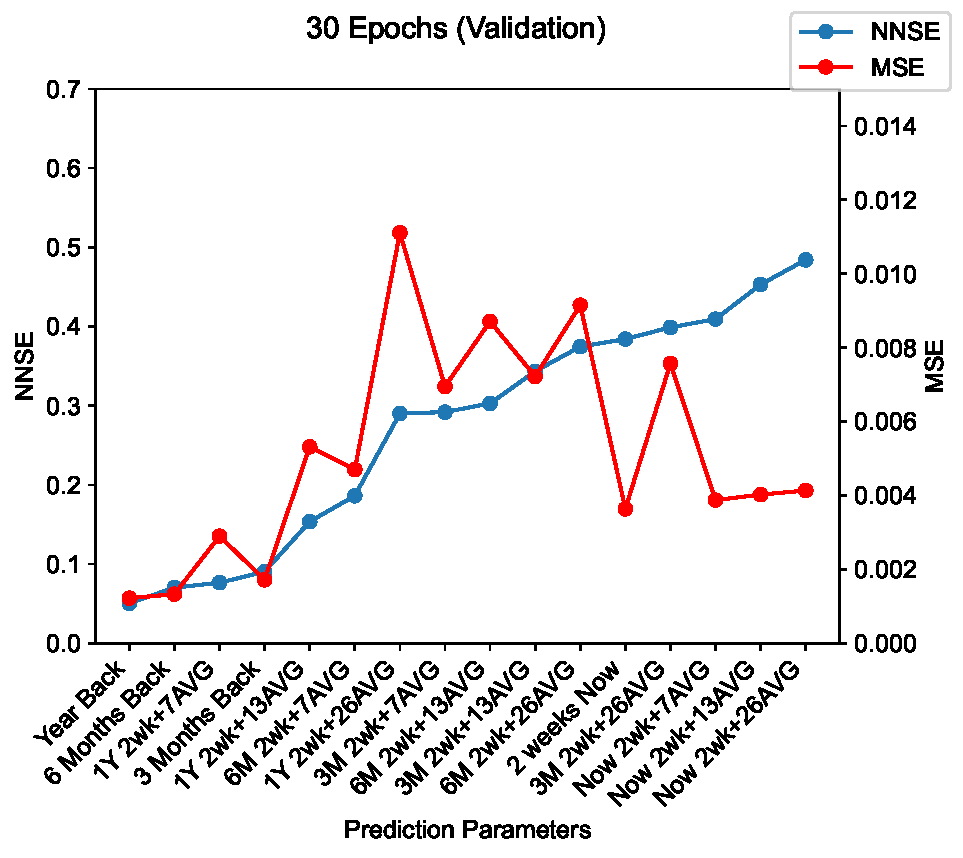
\includegraphics[width=1.0\linewidth]{images/30_validation-MSE-and-NNSE.pdf}
        \caption{MSE and NNSE - 30 epochs validation}
        \label{fig:tbd4}
     \end{subfigure}
     \hfill
          \newline
     \hfill
     \begin{subfigure}[b]{0.49\textwidth}
        \centering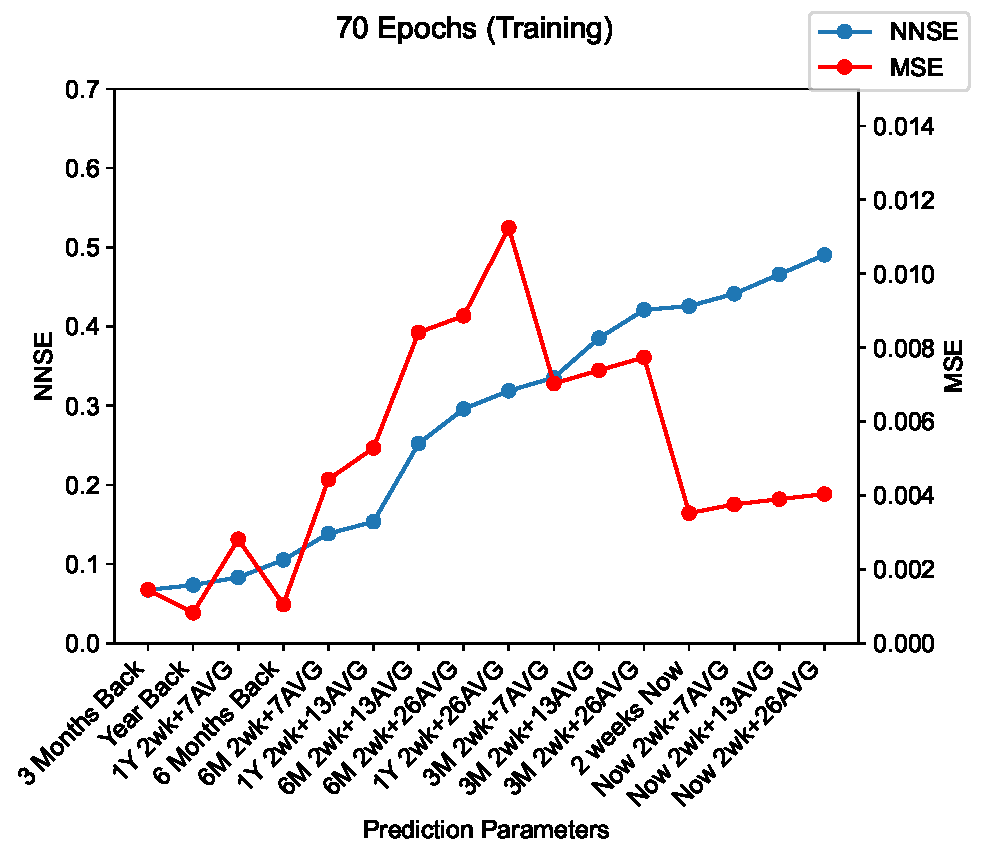
\includegraphics[width=1.0\linewidth]{images/70_training-MSE-and-NNSE.pdf}
        \caption{MSE and NNSE - 70 epochs training}
        \label{fig:tbd3}
     \end{subfigure}
     \hfill
     \begin{subfigure}[b]{0.49\textwidth}
        \centering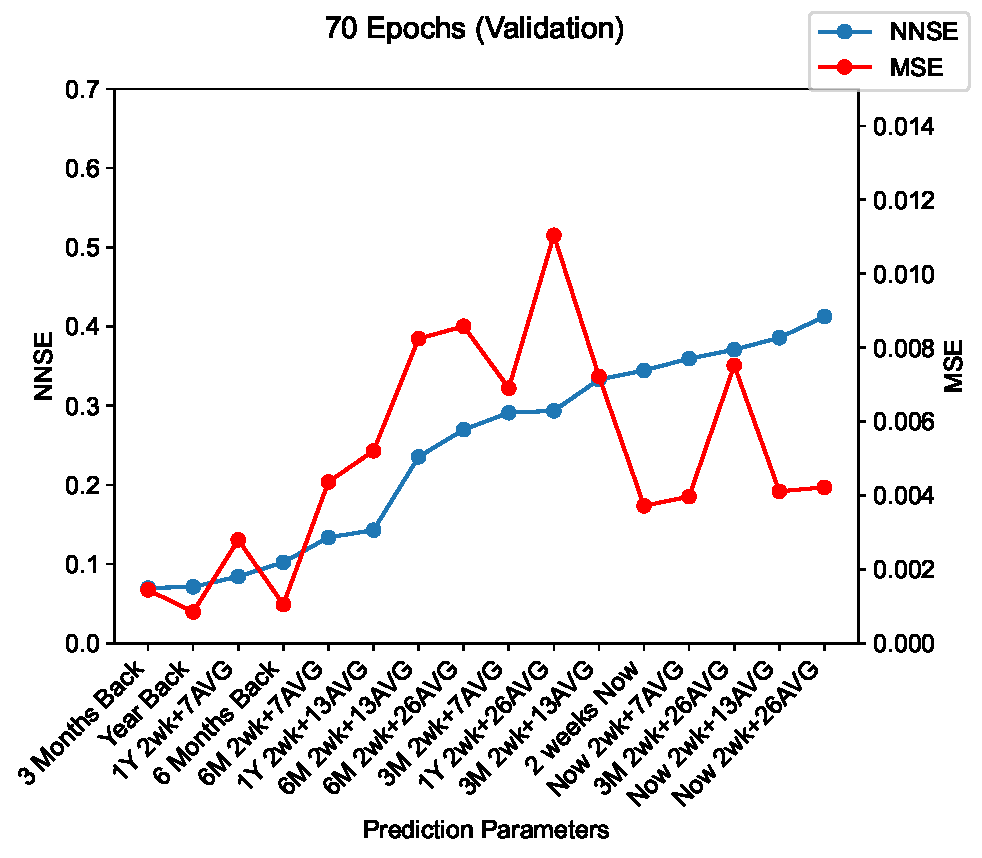
\includegraphics[width=1.0\linewidth]{images/70_validation-MSE-and-NNSE.pdf}
        \caption{MSE and NNSE - 70 epochs validation}
        \label{fig:tbd4}
     \end{subfigure}
        \caption{NNSE and MSE values for epochs 2, 30, 70 (training and validation).}
        \label{fig:six graphs}
\end{figure}

\end{comment}

\begin{comment}
\begin{table}[!h]

  \caption{Training}
\label{tab:training}
  
\begin{tabular}{rl}
NNSE & Name \\
\hline
0.191300 & Year Back \\
0.192700 & 6M 2wk+7AVG \\
0.197000 & 6M 2wk+13AVG \\
0.201600 & 6 Months Back \\
0.232600 & 1Y 2wk+13AVG \\
0.233000 & 3 Months Back \\
0.235800 & 1Y 2wk+7AVG \\
0.243000 & 3M 2wk+7AVG \\
0.251600 & 1Y 2wk+26AVG \\
0.251700 & 6M 2wk+26AVG \\
0.278800 & 3M 2wk+13AVG \\
0.302500 & 3M 2wk+26AVG \\
0.405600 & Now 2wk+7AVG \\
0.429900 & Now 2wk+13AVG \\
0.506800 & 2 weeks Now \\
0.521800 & Now 2wk+26AVG \\
\hline
\end{tabular}


\caption{valitation}
\label{tab:validation}

\begin{tabular}{rl}
NNSE & Name \\
\hline
0.195200 & 6M 2wk+7AVG \\
0.201000 & 6 Months Back \\
0.201600 & 6M 2wk+13AVG \\
0.204500 & Year Back \\
0.219700 & 3 Months Back \\
0.228900 & 3M 2wk+7AVG \\
0.238200 & 1Y 2wk+13AVG \\
0.249500 & 1Y 2wk+7AVG \\
0.264400 & 6M 2wk+26AVG \\
0.266200 & 3M 2wk+13AVG \\
0.270300 & 1Y 2wk+26AVG \\
0.295800 & 3M 2wk+26AVG \\
0.379700 & Now 2wk+7AVG \\
0.412700 & Now 2wk+13AVG \\
0.470100 & 2 weeks Now \\
0.502300 & Now 2wk+26AVG \\
\hline
\end{tabular}

\end{table}

\end{comment}

\end{document}
